
%\title{Error Correction in a Phenomenological Fibonacci Anyon Quantum Code}
\title{Random Fibonacci Anyons Simulable via Covariant Action of Mapping Class Group}

\author{Simon Burton, Courtney Brell, Steven Flammia}
%\date{\today}

\documentclass[12pt,a4paper]{article}
%\documentclass[11pt, twocolumn]{article}

%\usepackage[paper=a4paper,dvips,top=1.5cm,left=1.5cm,right=1.5cm,foot=1cm,bottom=1.5cm]{geometry}
\usepackage[paper=a4paper,dvips,top=3.0cm,left=1.5cm,right=1.5cm,foot=1cm,bottom=1.5cm]{geometry}

%\usepackage{epsf}
\usepackage{amsmath}
\usepackage{color}
\usepackage{natbib}
%\usepackage{cite}

\RequirePackage{amsmath}
\RequirePackage{amssymb}
\RequirePackage{amsthm}
%\RequirePackage{algorithmic}
%\RequirePackage{algorithm}
%\RequirePackage{theorem}
%\RequirePackage{eucal}
\RequirePackage{color}
\RequirePackage{url}
\RequirePackage{mdwlist}

\RequirePackage[all]{xy}
\CompileMatrices
\RequirePackage{hyperref}
\RequirePackage{graphicx}
\RequirePackage[dvips]{geometry}


\begin{document}

\maketitle

\def\Complex {C}
\def\tensor{\otimes}
\def\Tensor{\bigotimes}
\def\bra #1{\langle #1|}
\def\ket #1{|#1\rangle}
\def\braket #1#2{\langle #1|#2 \rangle}

%\def\Set{\widetilde{\text{Set}}}
%\def\Top{\widetilde{\text{Top}}}
%\def\Vec{\widetilde{\text{Vec}}}
%\def\Chain{\widetilde{\text{Chain}}}

%\def\ker{\text{ker}}
%\def\coker{\text{coker}}
%\def\im{\text{im}}

%\def\H{\mathcal{H}}
%\def\H{H}
%\def\S{S}
\def\mathZ{\mathbb{Z}}
\def\mathR{\mathbb{R}}

%\def\nin{\not\in}

%\def\heading #1{\noindent\underline{\Large\bf #1}}
\def\heading #1{\vskip 20pt \noindent\underline{\large \bf #1}\vskip 5pt}

\def\important #1{\underline{\bf #1}}

% ----------------------------------------------------------------------------
%

\heading{Braid group}

Braid group on $n$ strands is the group $B_n$ generated by $n-1$ generators
$\sigma_1, \sigma_2, ... \sigma_{n-1}$ with the following relations:
    $$ \sigma_i \sigma_j = \sigma_j \sigma_i \ \text{when}\ |i-j| > 2, $$
    $$ \sigma_i \sigma_{i+1} \sigma_i =  \sigma_{i+1} \sigma_i \sigma_{i+1}.$$


% ----------------------------------------------------------------------------

\heading{Fibonacci Anyons}

Every surface that is not a sphere, torus, disc or annulus, admits
a pair-of-pants decomposition, see \cite{Ivanov01}, Theorem 2.4.A.

So we have a (linear) representation of the braid group:

    $$ \kappa : B_n \to GL(F_n).$$

Where $F_n$ is the Hilbert state space of $n$ Fibonacci anyons with
trivial total charge.


% ----------------------------------------------------------------------------

\heading{Curve Diagrams}

The disc $D = \{ x\in \mathR^2\ s.t.\ |x|\leq 1 \} $,
has boundary $\partial D = \{ x\in \mathR^2\ s.t.\ |x|=1 \} $.

Given a finite set $ Q_n \subset D-\partial D$,
we denote $D_n$ as the pair $(D, Q_n).$
%Topologically, this definition does not depend on
%anything but the cardinality of $Q_n.$

We define the mapping class group of $D_n$,
$MCG(D_n),$ as the set of homeomorphisms $D\to D$ that
restrict to a permutation on $Q_n,$ modulo isotopy that
fixes $Q_n.$
Such an equivelance class
of homeomorphisms will be denoted as $\phi:D_n\to D_n.$

We can think of $D_n$ as the unit disc with $n$ holes,
and the mapping class group as the set of homeomorphisms on
this space, modulo isotopy.

The line $L = \{ x\in \mathR\ s.t.\ |x|\leq 1 \} $,
and a finite set $R_n\subset L$,
$L_n = (L, R_n).$
By a slight abuse of notation, we enumerate the points in $R_n$ 
in a monotonically increasing order,
and understand such notation as $[i, i+1]$ to mean the closed interval in $L$
with (consecutive) endpoints $i, i+1 \in R_n.$

We define a curve diagram as an embedding $f : L\to D$ that
restricts to a bijection $R_n\to Q_n,$ modulo
isotopy.
This will be denoted as $f : L_n\to D_n.$
We can generalize this to $f : L_m\to D_n$ with $m\leq n$
to mean a map $L\to D$ that restricts to an injection $R_m\to Q_n,$
modulo isotopy.

\begin{center}
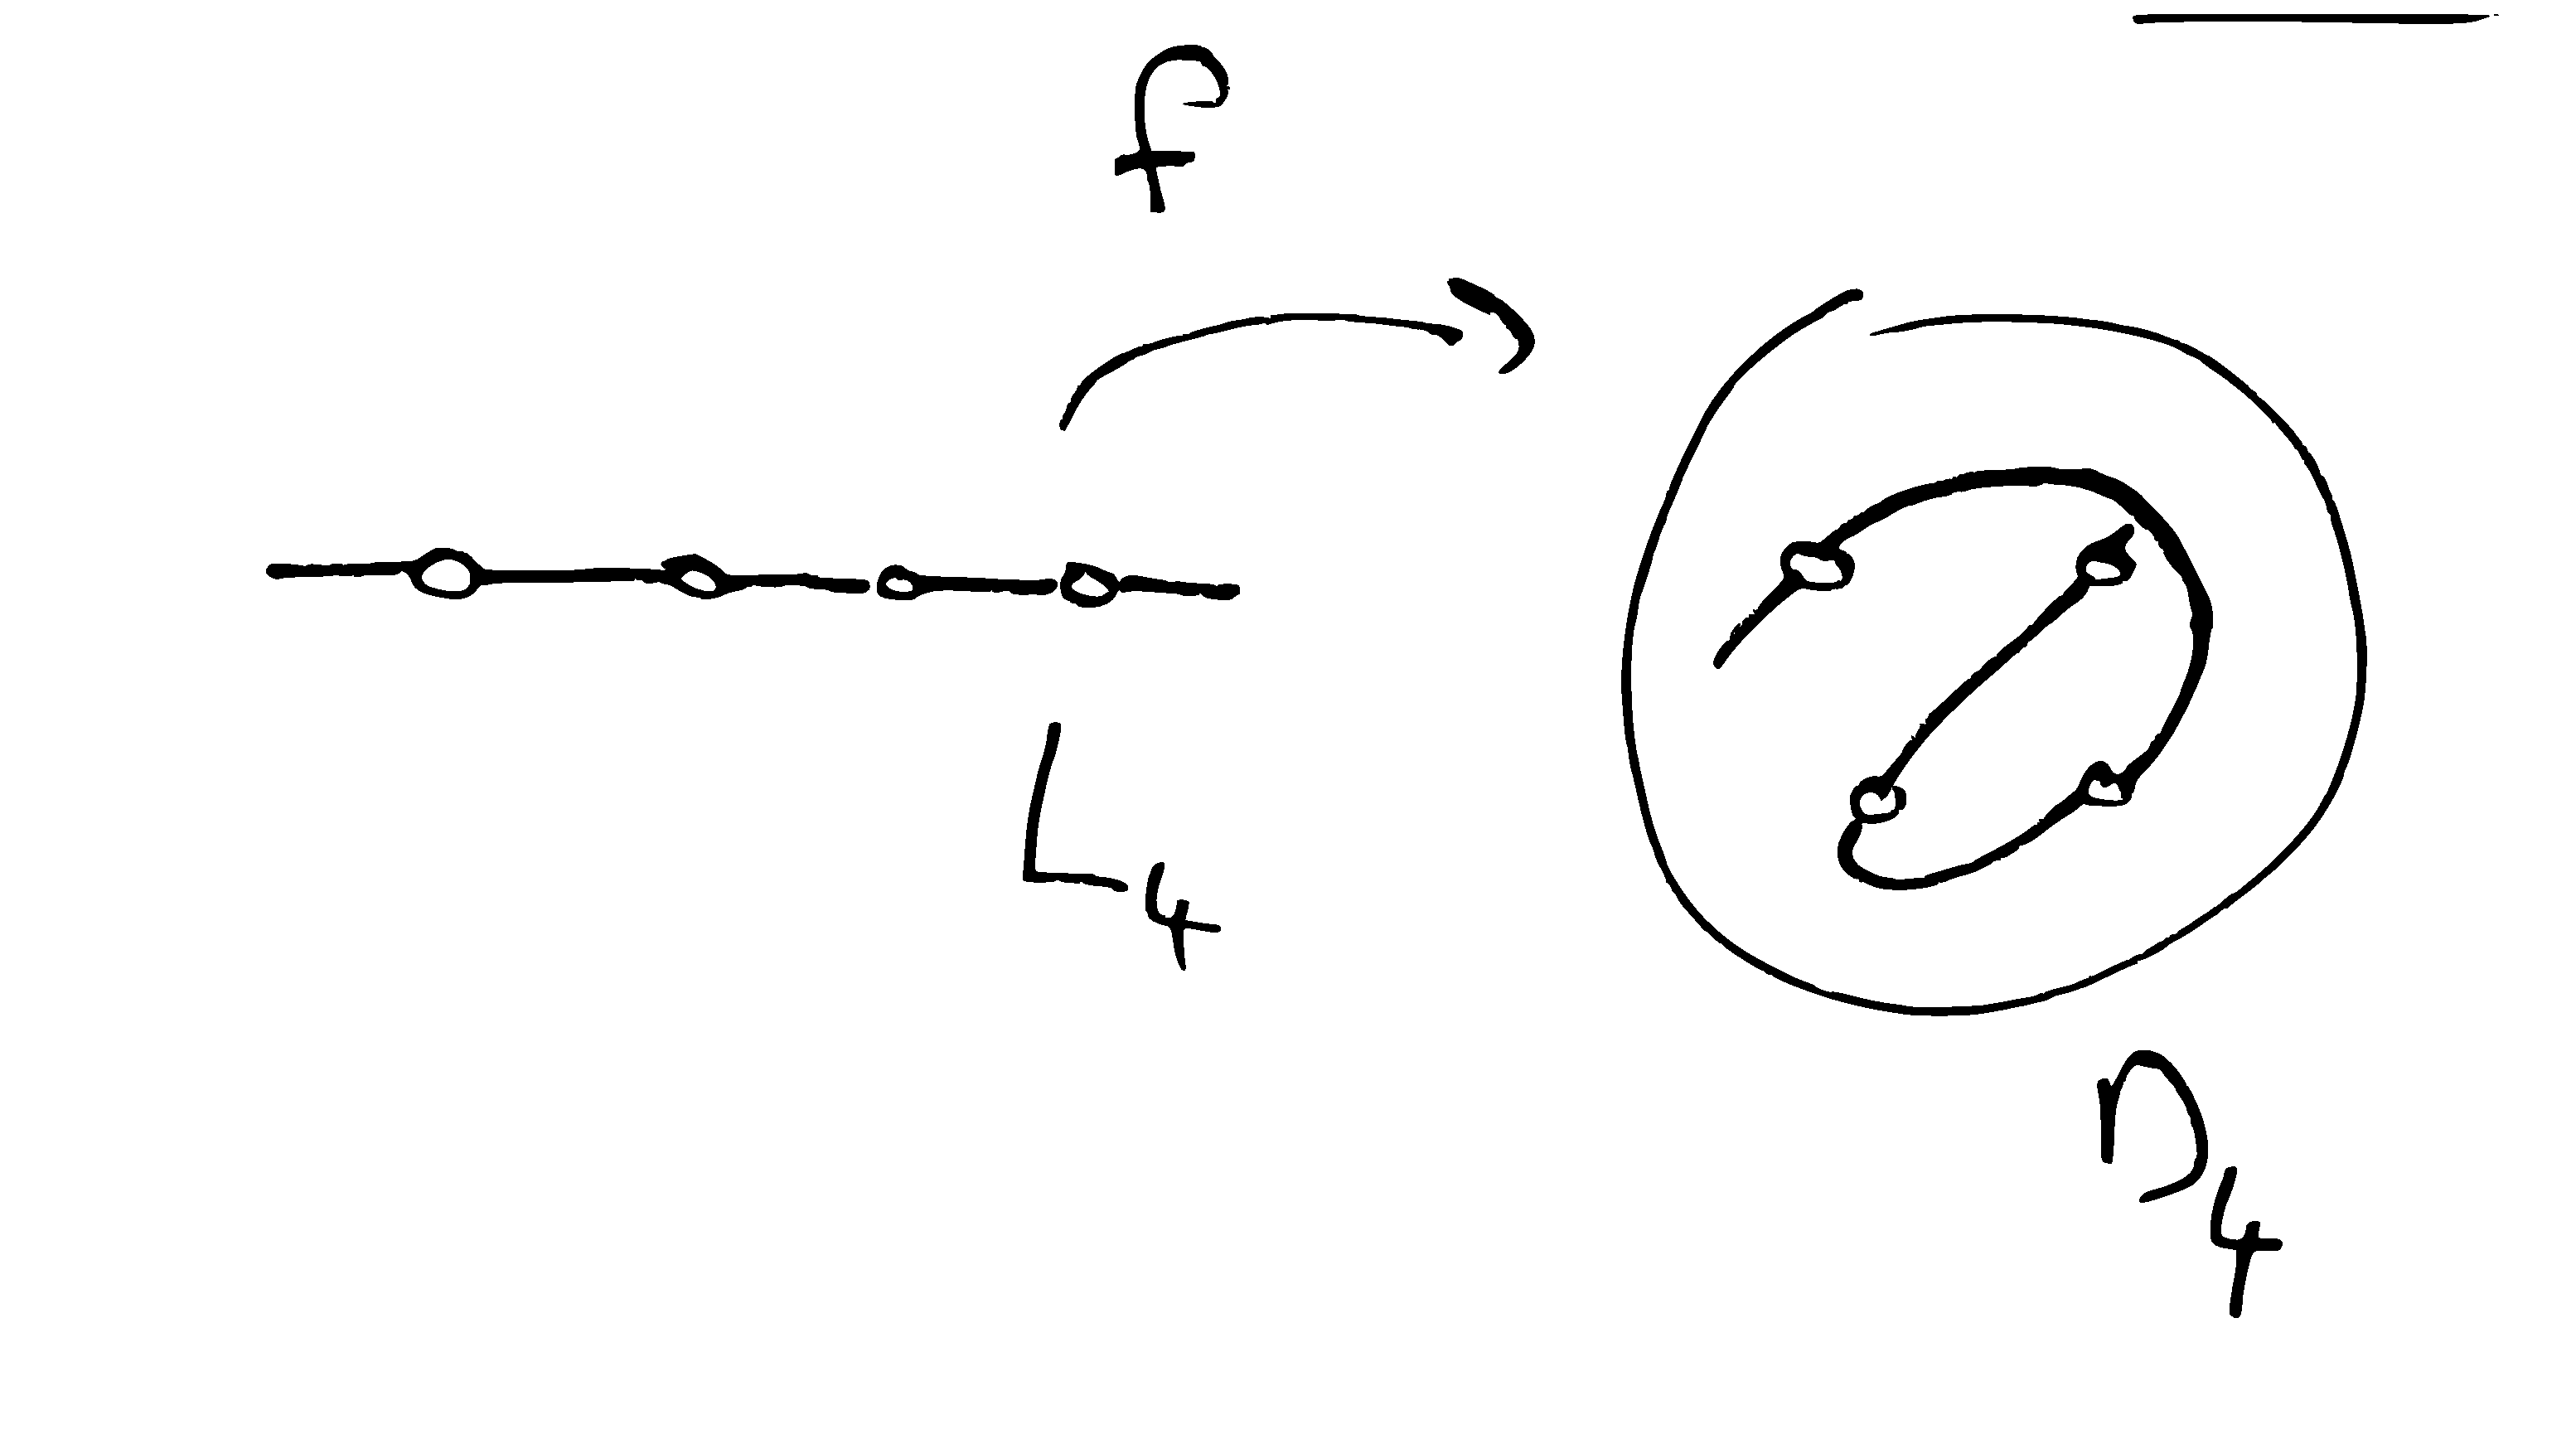
\includegraphics[width=0.5\textwidth]{curve-diagram.eps}
\end{center}


% ----------------------------------------------------------------------------

\heading{Group action}

The mapping class group $MCG(D_n)$ acts on curve diagrams $f : L_n\to D_n$
via post-composition (left multiplication). See \cite{Dehornoy02}, chapter 6.

%\heading{Braid group representation}

In particular, we can single out specific ``braid'' elements of $MCG(D_n)$.
These act on the image of a pair-of-pants embedding: $g:D_2\to D_n.$

DIAGRAM

Here we verify the braid relations directly:

\begin{center}
%\includegraphics[width=0.5\textwidth]{mypicture.png}
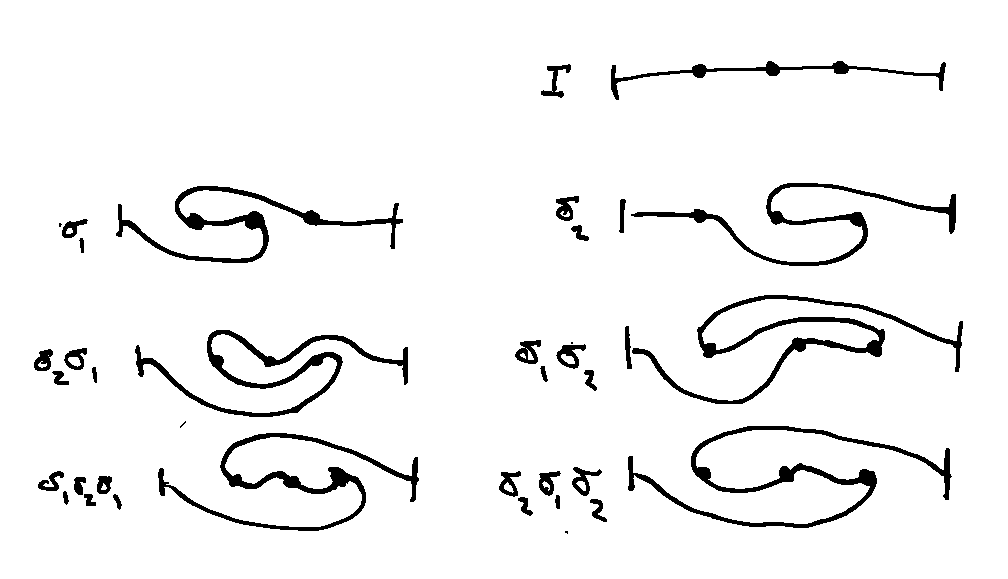
\includegraphics[width=0.5\textwidth]{curve-braid.eps}
\end{center}

% ----------------------------------------------------------------------------

\heading{Half-twists}

\important{Definition:} by a {\it half-twist} on a curve
diagram $f:L_n\to D_n$ at $i$ we mean an element of $MCG(D_n)$
that can be represented by a half-twist that acts
on a small neighbourhood of $f([i, i+1]).$
We denote a clockwise half-twist by $b(i, f):$

\begin{center}
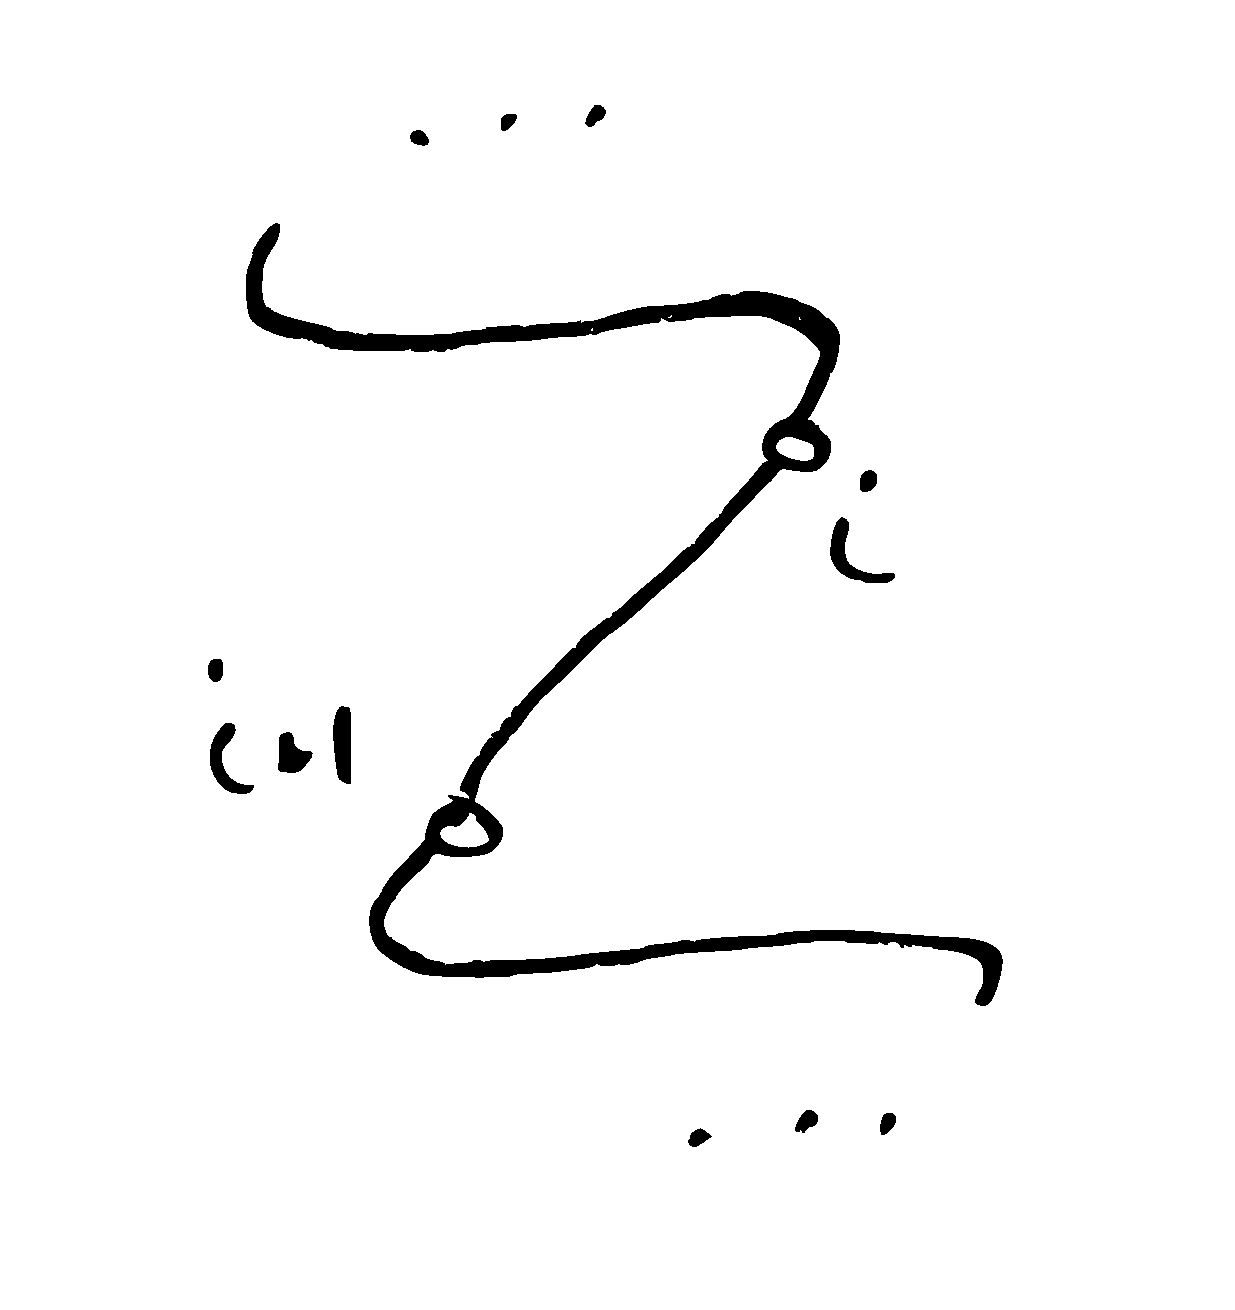
\includegraphics[width=0.2\textwidth]{halftwist-1.eps}
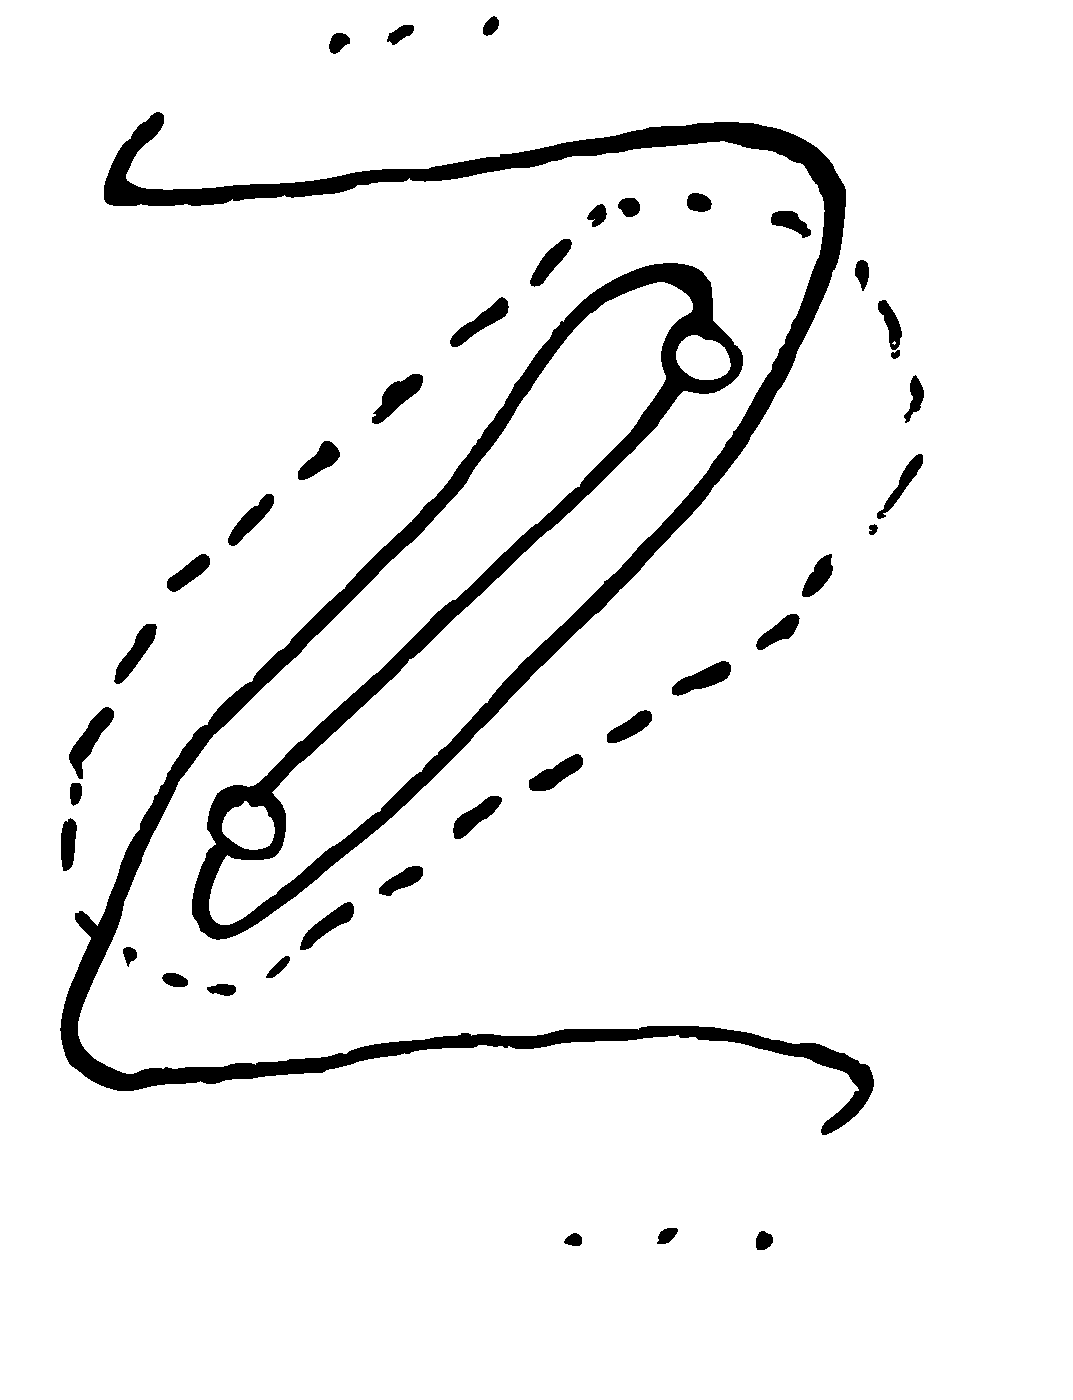
\includegraphics[width=0.15\textwidth]{halftwist-2.eps}
\end{center}

Each half-twist corresponds to a braid action of two neighbouring
holes on $f$.
See \cite{Kassel10}, Section 1.6.2, for more details on half-twists.

\important{Definition:} by a {\it sequence of half-twists} on a curve
diagram $f:L_n\to D_n$ we mean a
sequence of curve diagrams $f_k: L_n\to D_n$, and a sequence of half-twists:

        $$ b(i_1, f_1),\ b(i_2, f_2),\ ...\ b(i_N, f_N) $$

such that $f_1=f,$ and

        $$ f_{k+1} = b(i_k, f_k) f_k,\ \  \text{} 1\leq k<N.$$


% ----------------------------------------------------------------------------

\heading{Half-twist factorization of $MCG(D_n)$}

\important{Problem:}
Given curve diagrams $f:L_n\to D_n$ and $g:L_2\to D_n$
find $\phi\in MCG(D_n)$ as a product of
a sequence of half-twists such that
$g = \phi f i,$ where $i$ is an inclusion of $L_2$ into $L_n:$

\begin{center}
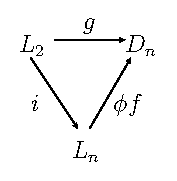
\includegraphics{halftwist-factor.eps}
\end{center}

The idea is that we would like to apply half-twists to a curve diagram
until the two holes indicated by $g$ become neighbours.

\important{Examples:}

In this example we use an inverse half-twist about the segment $[a, a+1]:$

\begin{center}
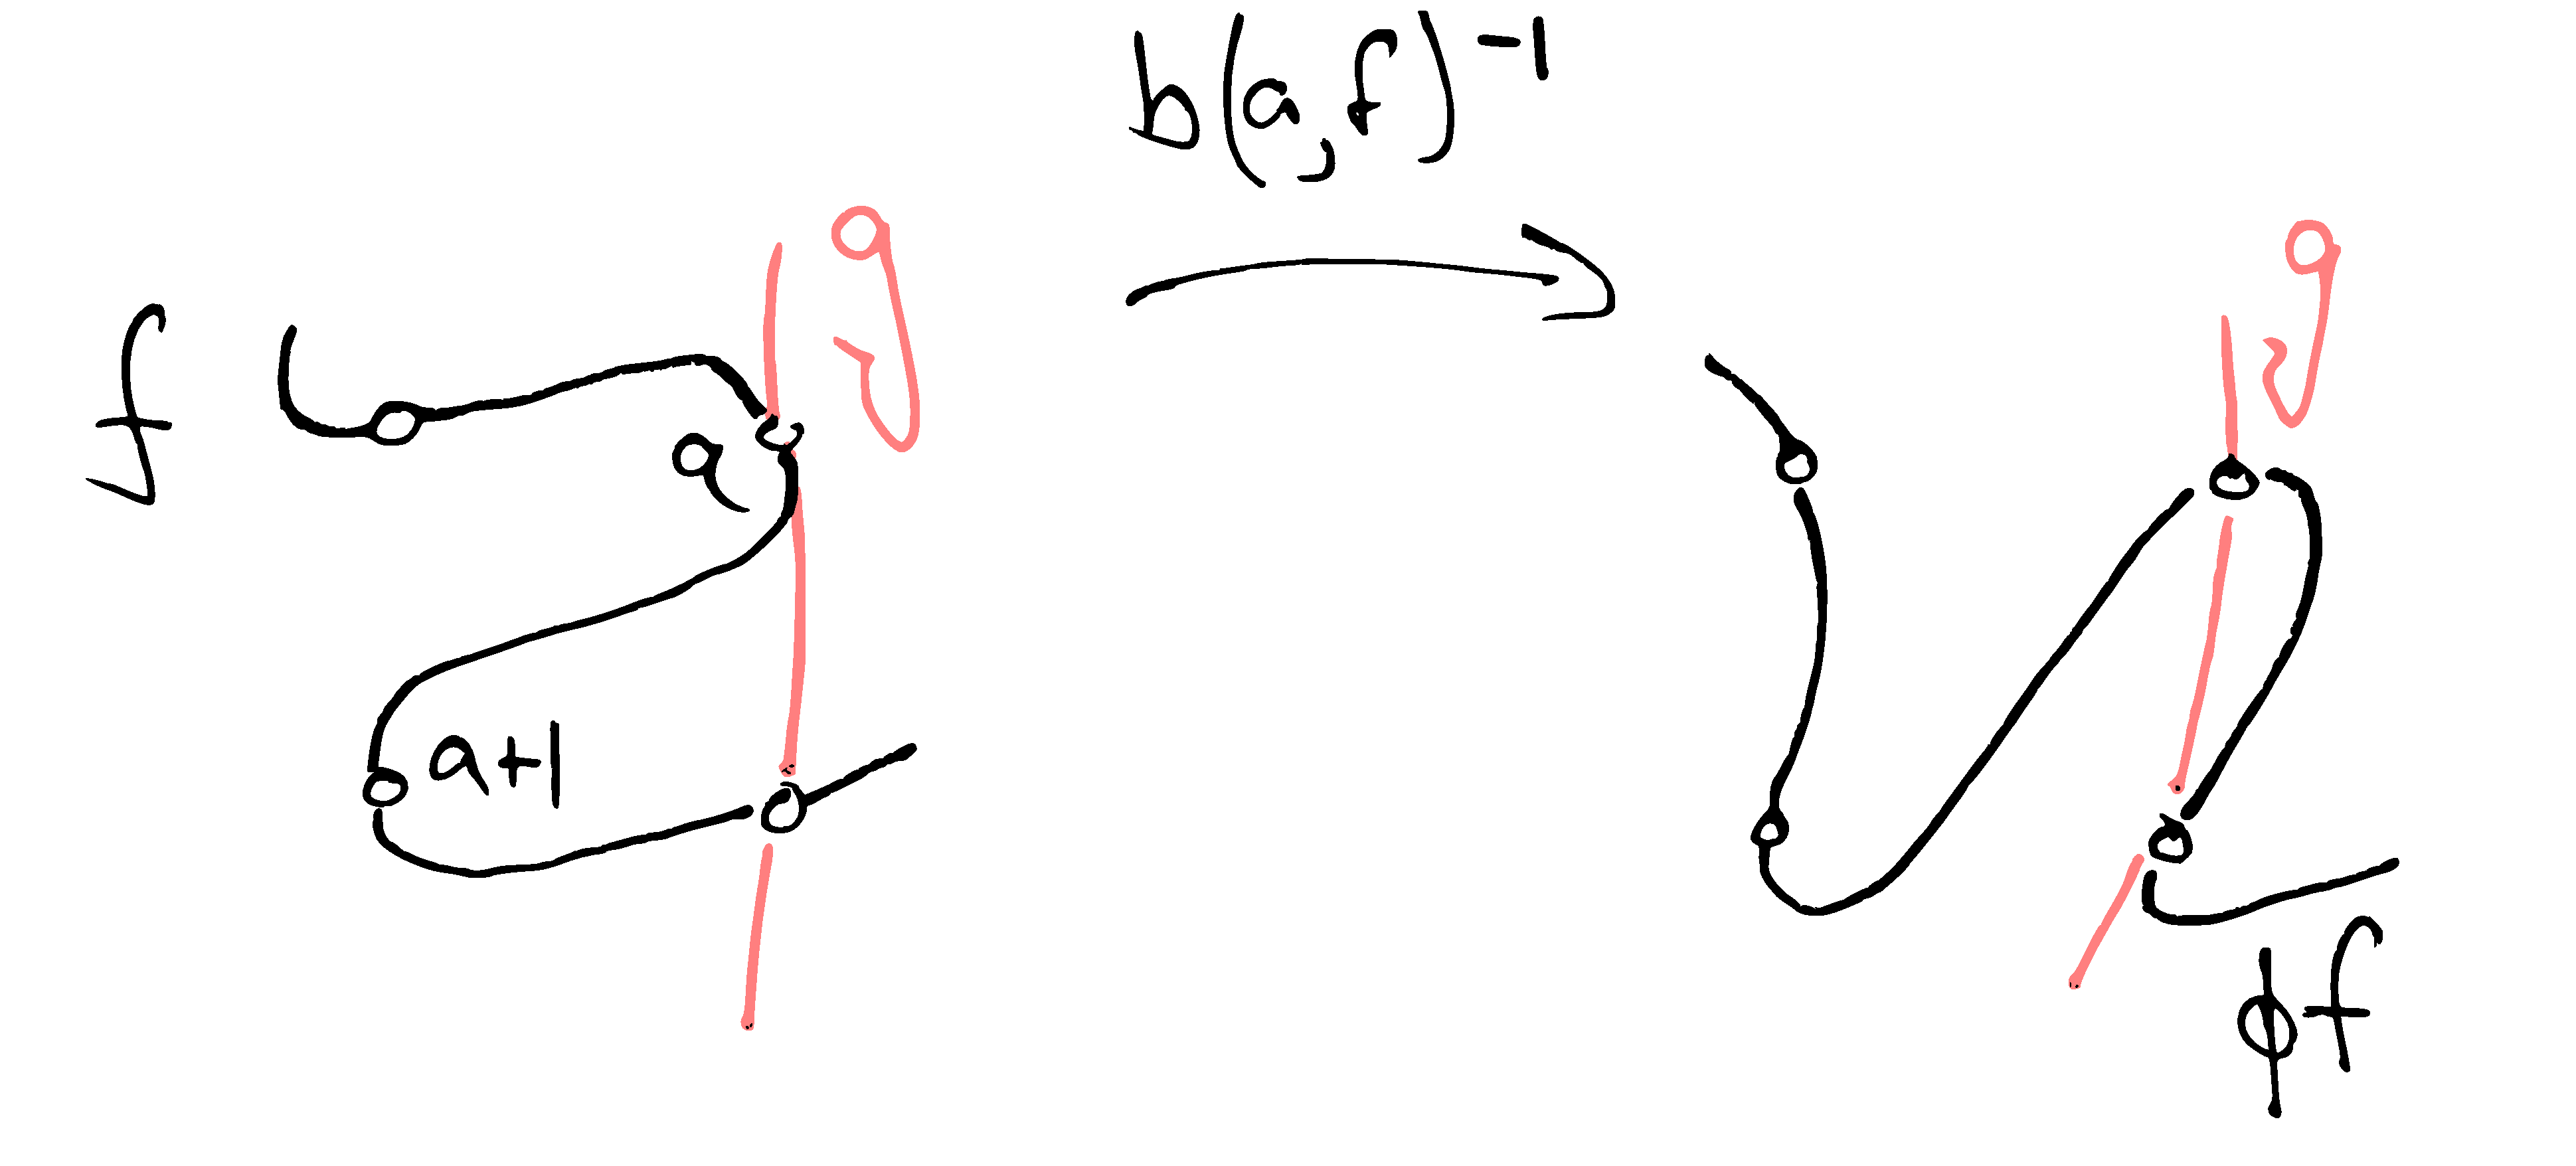
\includegraphics[width=0.6\textwidth]{example-problem-1.eps}
\end{center}


\important{Solution:}

1) decompose $f$ along (finitely many) intersections
with $g.$

\begin{center}
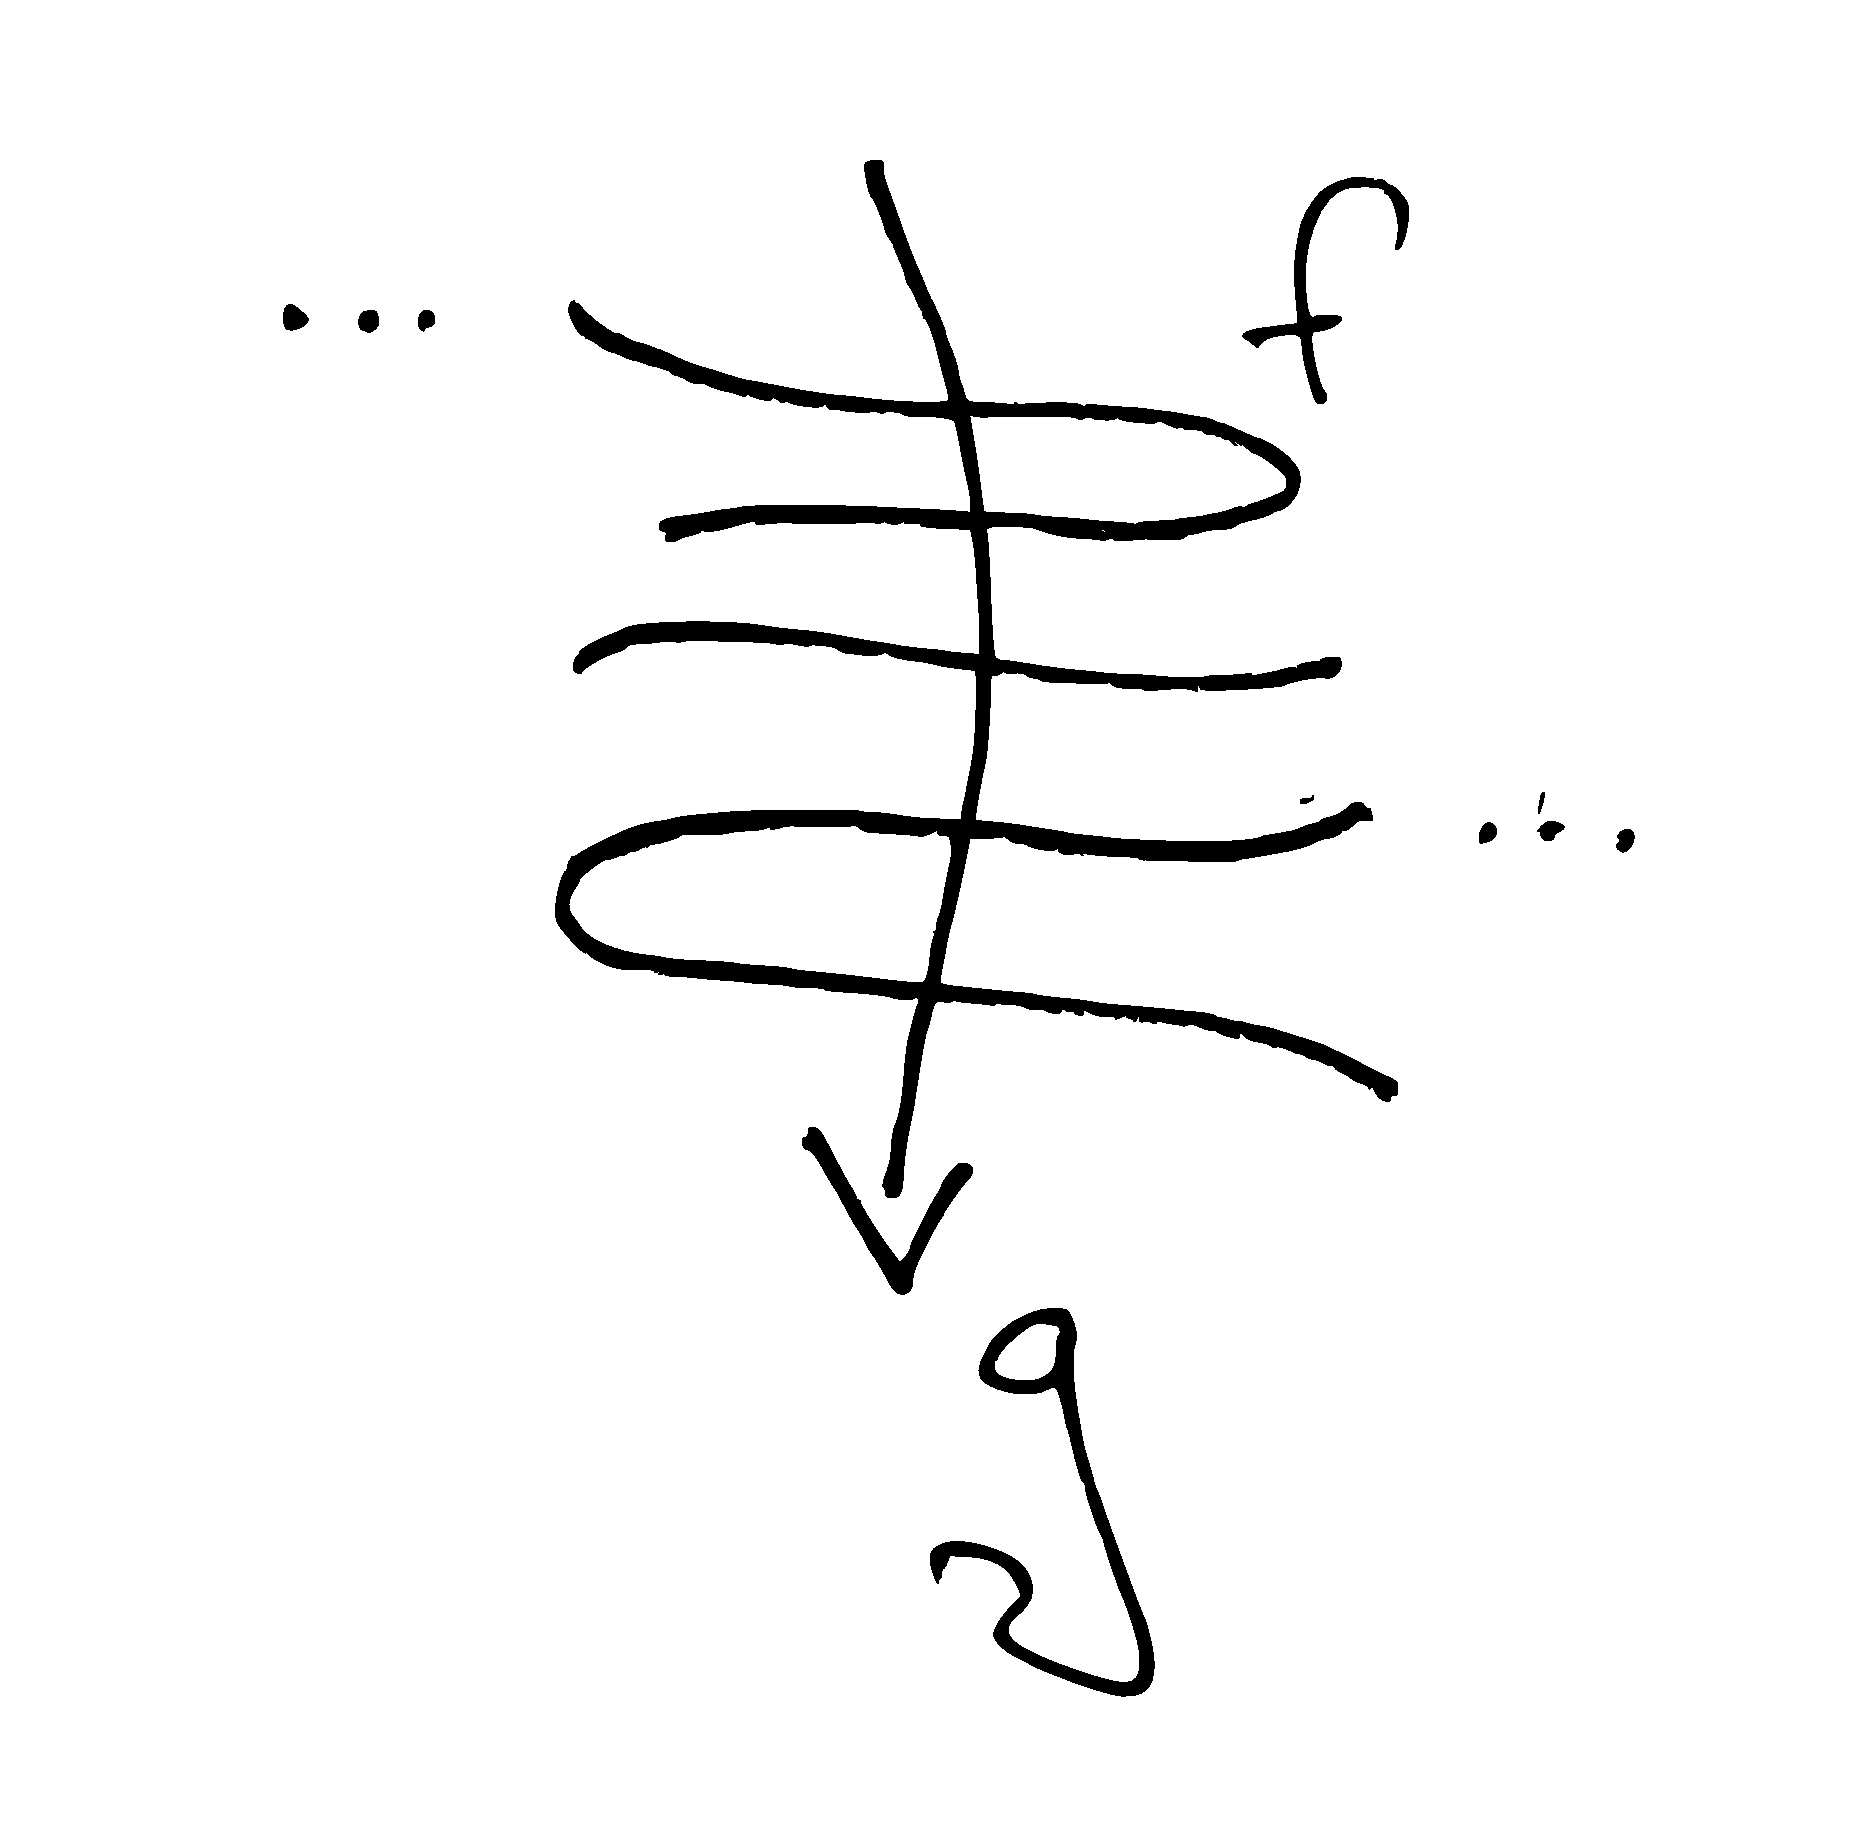
\includegraphics[width=0.3\textwidth]{snake-decompose.eps}
\end{center}


2) on each component $k$:

\begin{center}
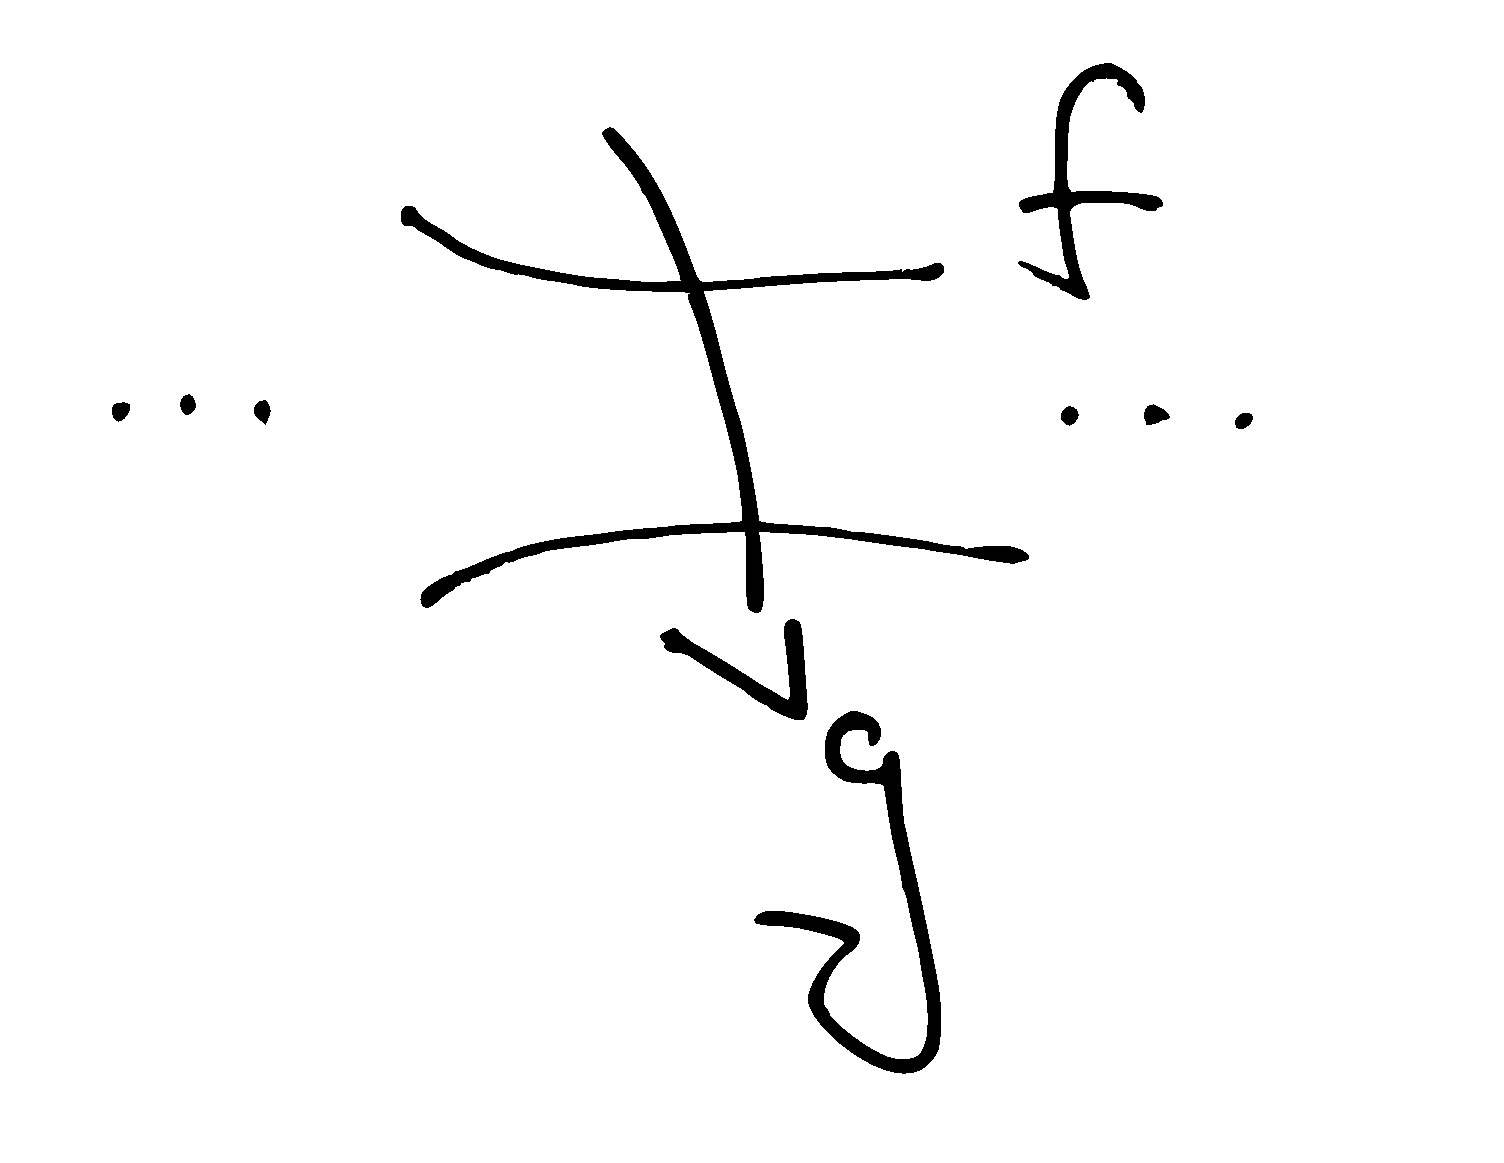
\includegraphics[width=0.3\textwidth]{snake-component.eps}
\end{center}

let $h_k = g_k + f_k.$
This is a simple closed curve in $D$ which splits $D$
into two regions, the inside (simply connected) and the
outside.
We find three basic cases (there are more including reflections
and rotations of these), which we can distinguish between
using the winding number and whether the end points
of $f$ are on the inside or outside of $h_k$:

\begin{center}
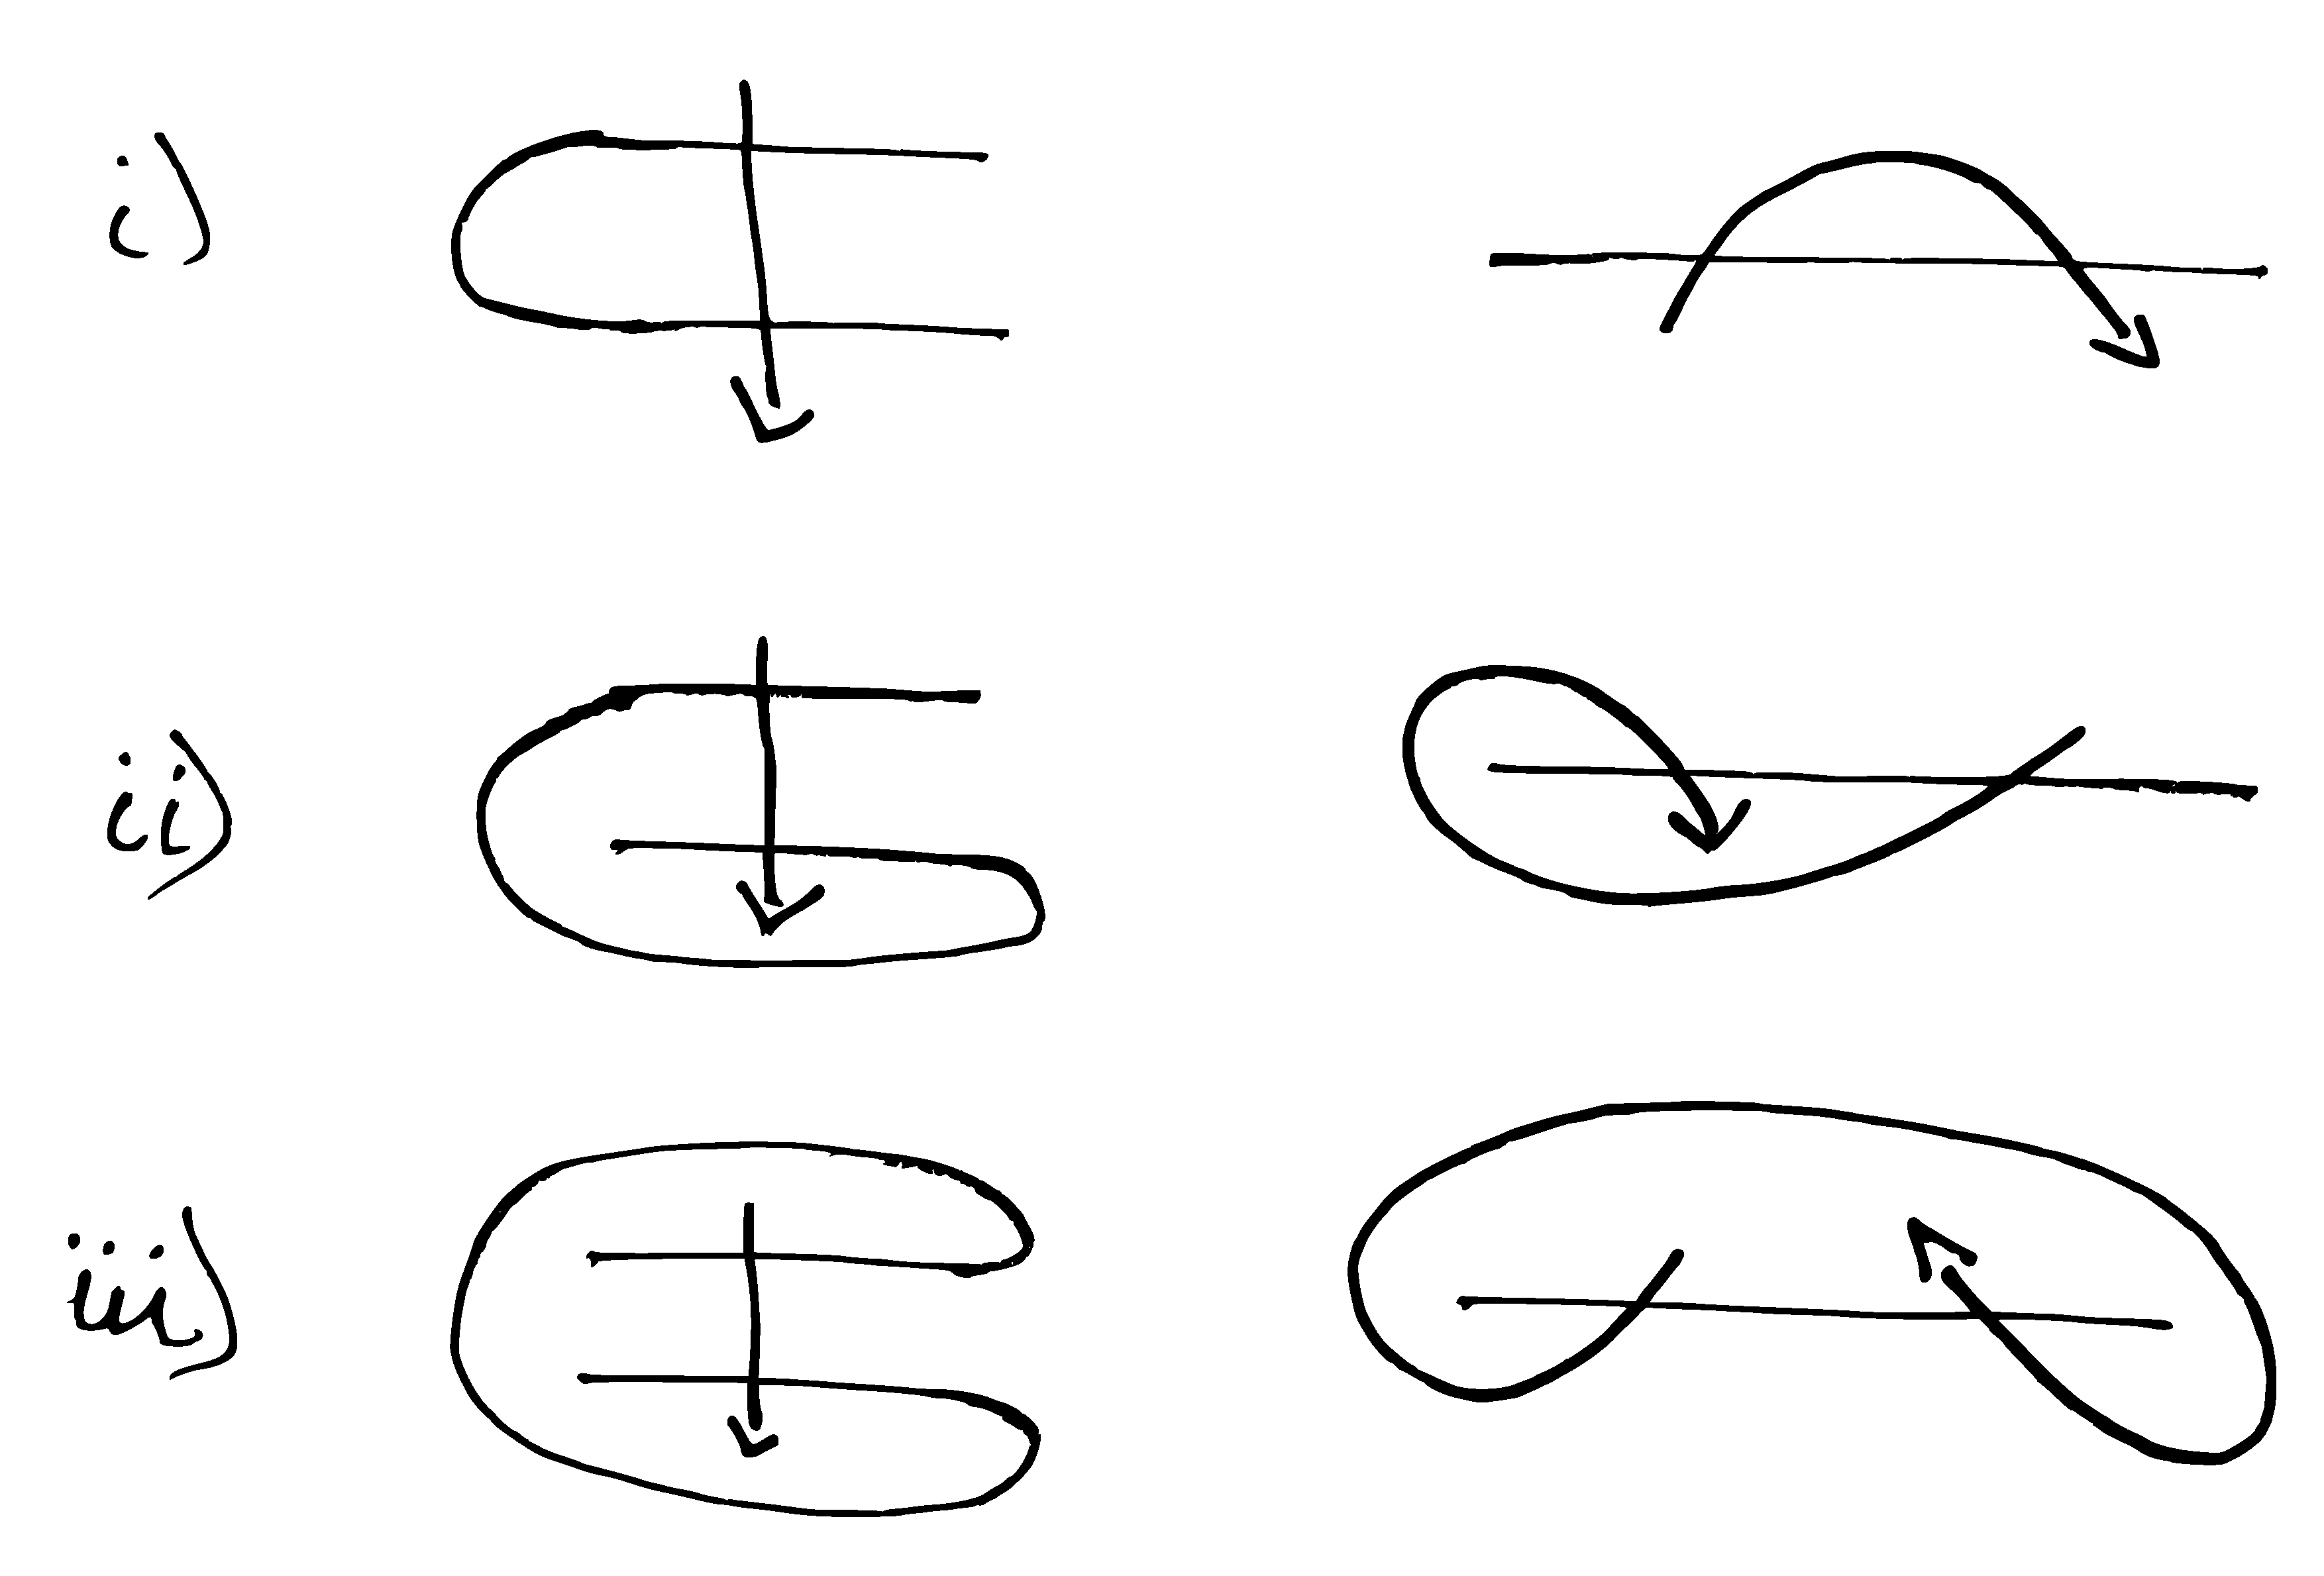
\includegraphics[width=0.5\textwidth]{snake-cases.eps}
\end{center}


% ----------------------------------------------------------------------------

\heading{Disjoint sum of two curve diagrams}

Given two disjoint curve diagrams $f:L_m\to D_n$ and $f':L_{m'}\to D_n$
we define their sum  $f+f':L_{m+m'}\to D_n$ ...


% ----------------------------------------------------------------------------

\heading{Planar diagrams}

We aim discretize the problem for software implementation.
Our first task is to characterize what happens to a curve
if we ``forget'' any braiding inside a disc.
We define the following set of ``planar diagrams'' as:

    $$ T = \{ f(L)\cap E / \sim \ \text{s.t.}\ f:L\to D \}$$

where $f:L\to D$ is a curve (not an isotopy class)
whose image $f(L)$ intersects a disc $E\subset D$ in a finite number of components
and the equivalence relation $\sim$ consists of isotopies that fix $\partial E.$

This object has a simple combinatorial description 
as a string consisting of
the four labels {\bf ( ) H T} such that 
the parentheses are balanced. The two labels H and T specify the
head and tail endpoints of $f$, and each appears at most once in the string.

For example, the following diagram is represented by
the string {\bf(())H}:

\begin{center}
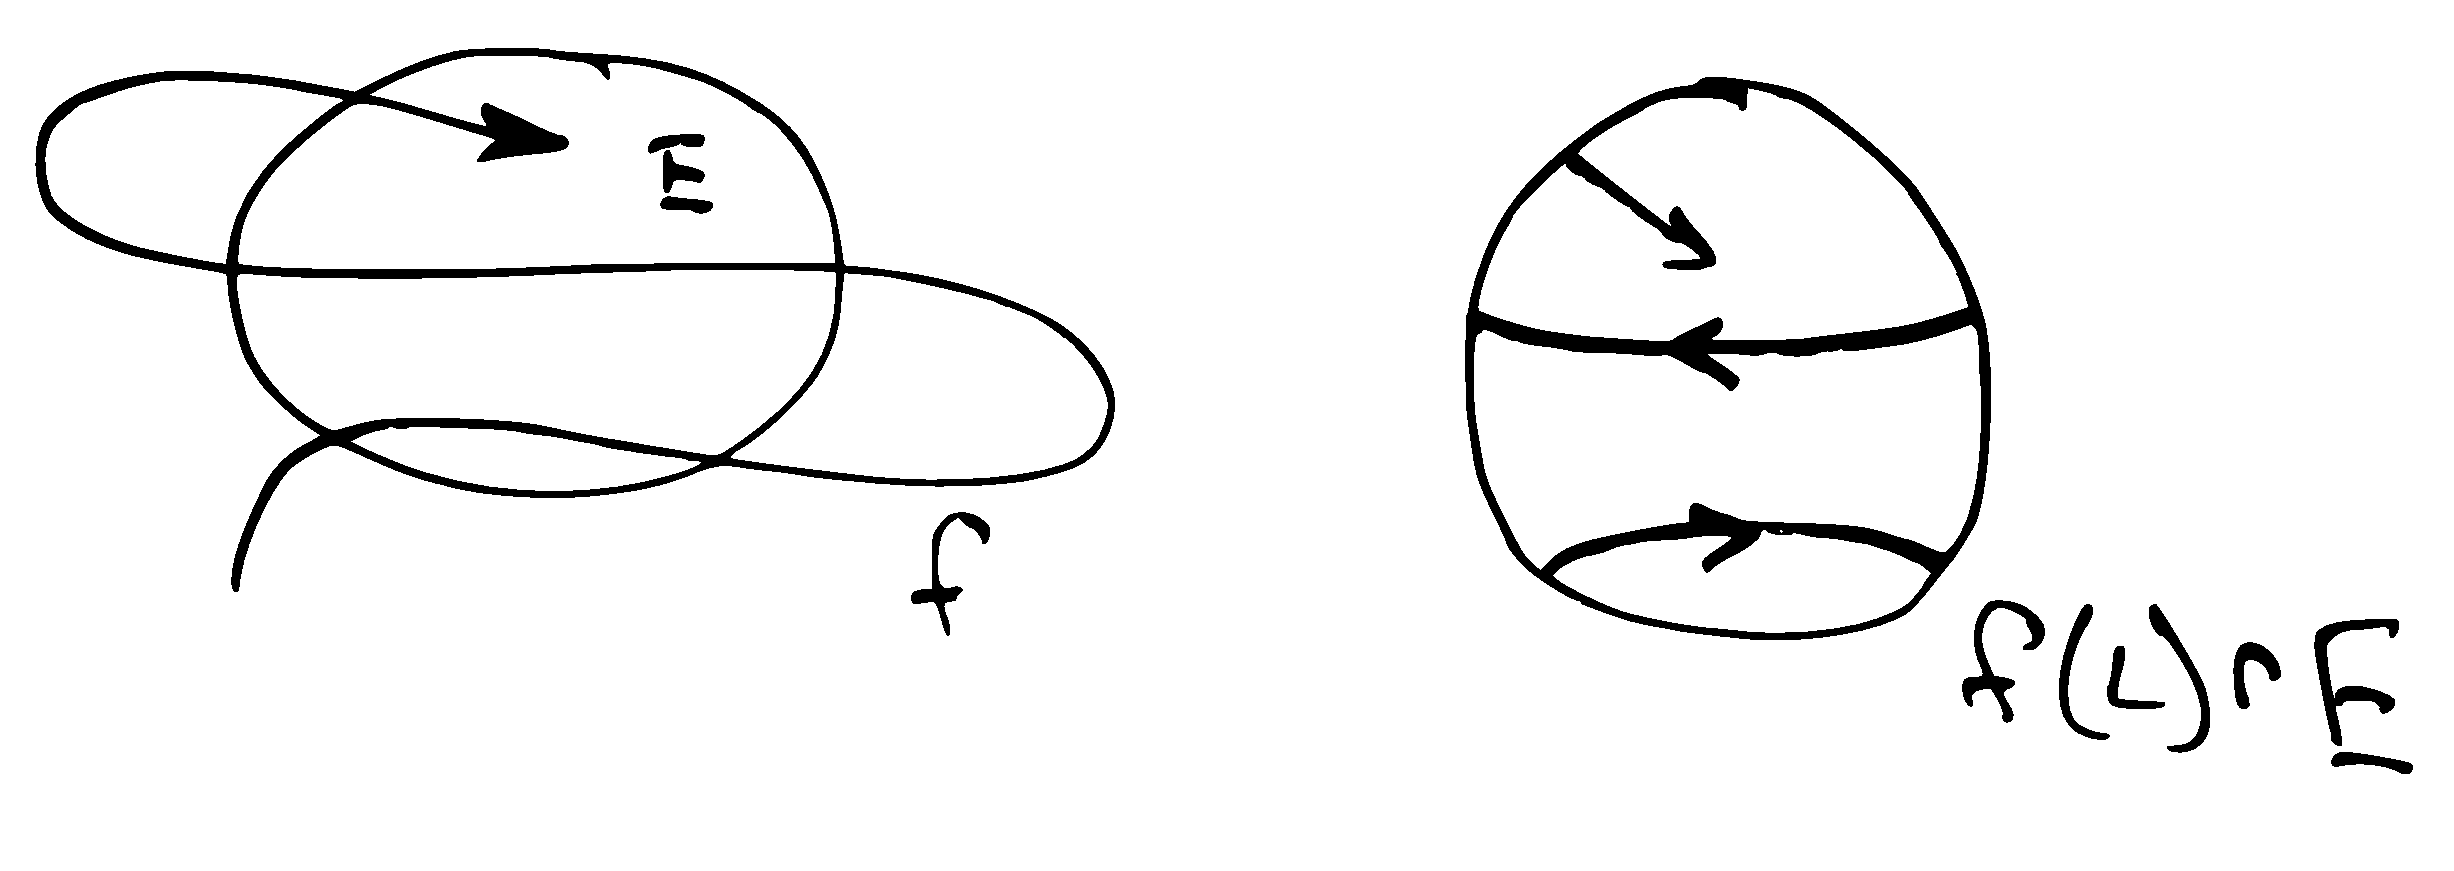
\includegraphics[width=0.5\textwidth]{planar.eps}
\end{center}

See \cite{Abramsky08} Proposition 1.6, for a similar treatment.

% ----------------------------------------------------------------------------

\heading{Tiling}

Now we consider a tiling of the disc into subdiscs that are disjoint on
their interiors.

% ----------------------------------------------------------------------------

\heading{Simulation and noise model}



% ----------------------------------------------------------------------------

\heading{Numerical results}

\begin{center}
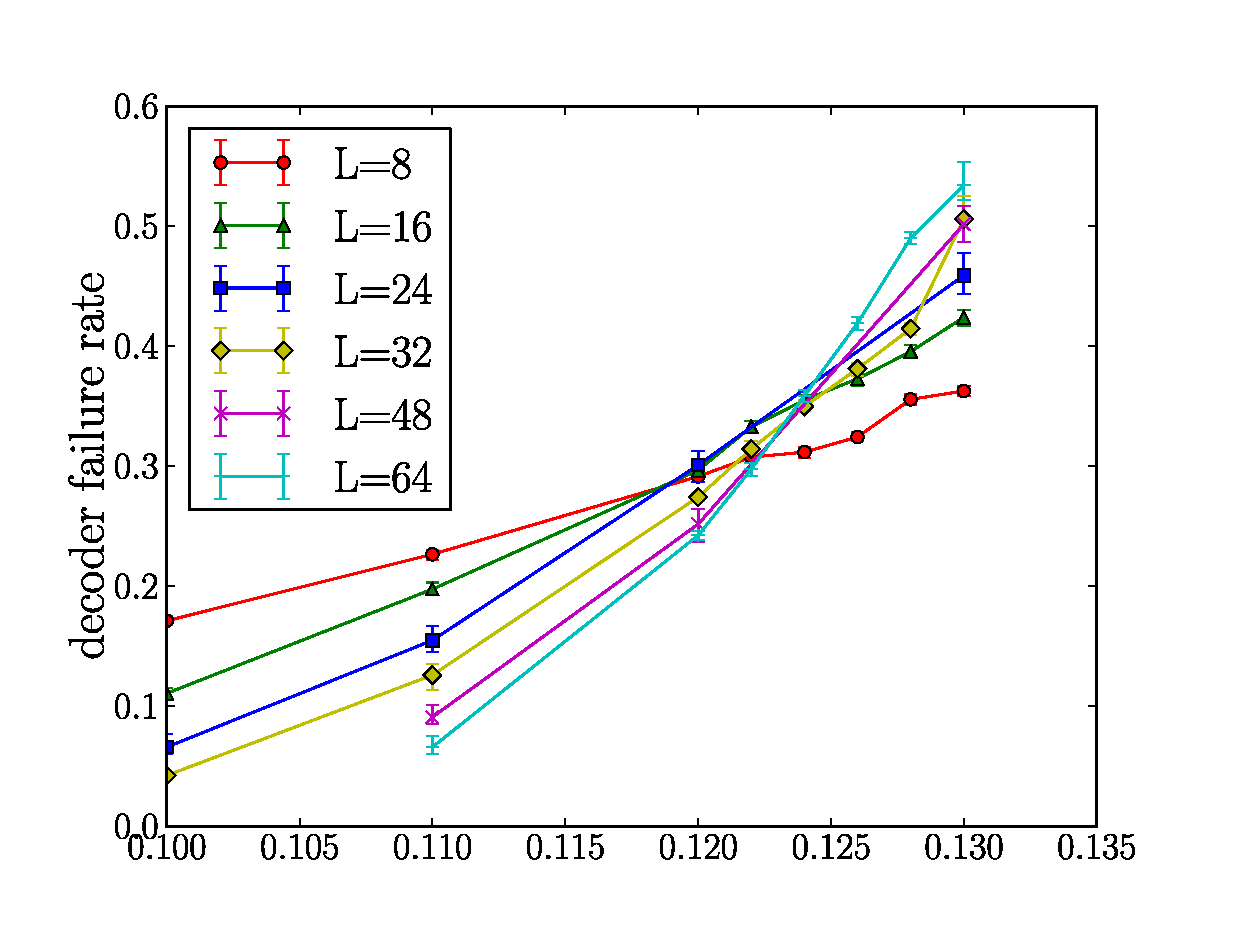
\includegraphics[width=0.5\textwidth]{threshold-graph.eps}
\end{center}

% ----------------------------------------------------------------------------

%Given a topological space $X$ we define the {\it mapping class group} of $X$ as
%the set of homeomorphisms $f:X\to X$ modulo isotopy
%
%    % $$ MCG(X) := \{ f : X \to X \text{s.t.} f \text{is homeomorphism} \} / \sim_{\text{iso}} $$
%    $$ MCG(X) := \{ f : X \to X \} / \sim_{\text{iso}}.$$

%Given a topological manifold $M$ we define the {\it mapping class group} of $M$ as
%the set of homeomorphisms $f:M\to M$ modulo isotopy
%
%    $$ MCG(M) := \{ f : M \to M \} / \sim_{\text{iso}}.$$
%
%If $M$ has boundary $\partial M$ we require the homeomorphisms to
%be the identity on $\partial M$.
%
%In particular we are interested in
% the $n$-punctured disc.
%This is a disc $D = \{ x\in \mathR^2 s.t. |x|\leq 1 \} $
%with $n$ points removed:
%
%    $$ D_n := D - Q_n,$$
%
%where $Q_n$ is some finite subset of the interior of $D$.
%
%%topologically this is a sphere with $n+1$ holes in it.
%
%It is a theorem that the group $MCG(D_n)$ is isomorphic to $B_n.$
%(See \cite{Kassel10}, chapter 1.)
%
%We fix $Q_n$ to be the points $\{(0, i/(n+1)) for i=1,...n\}$
%then we define the line $L = \{(0, x) s.t. |x|\leq 1\}.$
%Given a representative $f$ of an element of $MCG(D_n)$
%we define the
%curve diagram as the
%image of $L$ under $f$.
%
%It is a theorem (see \cite{Dehornoy02}) that such curve diagrams
%correspond uniquely to elements of the mapping class group, and
%hence to the braid group $B_n$.

% ----------------------------------------------------------------------------

%\heading{Pair-of-pants decompositions}

%We measure charge in regions bounded by curves, ie. elements of
%the first homology group $H_1(D_n).$


%http://arxiv.org/pdf/1002.2816.pdf
%http://www.math.ucsb.edu/~zhenghwa/data/course/lecture_notes/Chap2.pdf
%http://physics.stackexchange.com/questions/93183/about-the-atiyah-segal-axioms-on-topological-quantum-field-theory
%http://mathoverflow.net/questions/359/a-reading-list-for-topological-quantum-field-theory
%http://projecteuclid.org/download/pdf_1/euclid.cmp/1104178138
%http://arxiv.org/pdf/math/9912085v1.pdf


%% ----------------------------------------------------------------------------
%
%\heading{Combinatorial Formulation}
%
%% ----------------------------------------------------------------------------
%
%\heading{Numerical Simulations}

% ----------------------------------------------------------------------------

\bibliography{refs}{}
\bibliographystyle{abbrv}

\end{document}


